\documentclass[openany]{book}
%\setlength{\oddsidemargin}{0.in}
%\setlength{\textwidth}{6.5in}
%\setlength{\topmargin}{-0.25in}
%\setlength{\textheight}{8.25in}

% Skip space between paragraphs
\setlength{\parskip}{.1in}

% Do not put numbers in section headings
\setcounter{secnumdepth}{0}

% Indent paragraphs 0. in
\setlength{\parindent}{0.in}

% Use the natbib package for the bibliography
\usepackage[round]{natbib}
\bibliographystyle{sysbio}

% Use the graphicx package to incorporate and scale
% encapsulated postscript figures
\usepackage{graphicx}

% Make document single-spaced
\renewcommand{\baselinestretch}{1.0}

\newcommand{\summarysymbol}{$\hookrightarrow$}

\usepackage{wrapfig}

%\usepackage{float}
%\floatstyle{plain}
%\newfloat{floatbox}{!hb}{loa}
%w3\floatname{floatbox}{Box}

\newcounter{aside}
\newenvironment{aside}[2]
{
	\label{#1}
	\stepcounter{aside}
	%\begin{floatbox}
	\begin{centering}
	\hfill \begin{tabular}{c} \hline \hline
	\\
	\begin{minipage}{5.in}
	\small {\bfseries Box~\arabic{aside}: #2} --- 
}
{
	\end{minipage} \\ \\ \hline \hline
	\end{tabular} \hfill
	\end{centering}
	%\end{floatbox}
}

\setlength{\oddsidemargin}{0.75in}
\setlength{\evensidemargin}{0.in}
\setlength{\textwidth}{5.75in}
\setlength{\parindent}{0.in}

%\newfont{\msamsix}{MSAM10 at 6pt}
%\newfont{\mmlfnt}{eurb10 at 10pt}
%\newfont{\mmlfntlg}{eurb10 at 18pt}

% use the fancyhdr package to allow both headers and footers
\usepackage{fancyhdr}
\pagestyle{fancy}
\fancyhf{} % clear all headers and footers
\fancyhead[LO,RE]{Phycas Developer Guide}
\fancyhead[RO,LE]{\thepage}
\fancyfoot[LO,LE]{{\footnotesize \copyright\ 2008 by Paul O. Lewis, Mark T. Holder and David L. Swofford}}
\fancyfoot[CE,CO]{}

% chapter pages will be in plain pagestyle, so we need to redefine
% the plain pagestyle to have the same format as other pages
\fancypagestyle{plain}{%
\fancyhf{} % clear all headers and footer fields except those redefined below
\fancyhead[LO,RE]{Bayesian Phylogenetics From the Ground Up}
\fancyhead[RO,LE]{\thepage}
\fancyfoot[LO,LE]{{\footnotesize \copyright\ 2007 by Paul O. Lewis, Mark T. Holder and David L. Swofford}}}

\newcommand{\Phycas}{{\sf Phycas}}
\newcommand{\phycas}{{\sf Phycas}}
\newcommand{\microsoft}{Microsoft$^{\mbox{\msamsix r}}$}
\newcommand{\winthirtytwo}{Win32$^{\mbox{\msamsix r}}$}
\newcommand{\windows}{Windows$^{\mbox{\msamsix r}}$}

\newcommand{\treeviewurl}{{\tt http://taxonomy.zoology.gla.ac.uk/rod/treeview.html}}
\newcommand{\lewislabsurl}{{\tt http://lewis.eeb.uconn.edu/lewishome/}}
\newcommand{\nclurl}{{\tt http://sourceforge.org/projects/ncl/}}

\newcommand{\ba}{\begin{array}}
\newcommand{\ea}{\end{array}}

\newcommand{\be}{\begin{eqnarray*}}
\newcommand{\ee}{\end{eqnarray*}}

\newcommand{\bi}{\begin{itemize}}
\newcommand{\ei}{\end{itemize}}

\newcommand{\rr}{{\rho}}
\newcommand{\rrr}{{\rho_r}}
\newcommand{\Lmprime}{{L'_m}}
\newcommand{\Lmdblprime}{{L''_m}}

\newcommand{\Lconditional}{ \mbox{$\L$} }
\newcommand{\Lmconditional}{ \mbox{$\L_m$} }
\newcommand{\Lmconditionalprime}{ \mbox{$\L'_m$} }
\newcommand{\Lmconditionaldblprime}{ \mbox{$\L''_m}$ }

\newcommand{\Lconst}{ \mbox{$L_{\star}$} }
\newcommand{\Lconstprime}{ \mbox{$L'_{\star}$} }
\newcommand{\Lconstdblprime}{ \mbox{$L''_{\star}$} }

\newcommand{\term}[1]{{\bfseries #1}}
\newcommand{\pathname}[1]{{\em #1}}
\newcommand{\class}[1]{{\tt #1}}
\newcommand{\variable}[1]{{\tt #1}}
\newcommand{\shptr}[1]{{\tt #1}}
\newcommand{\method}[1]{{\tt #1}}

%\newenvironment{box}{\begin{centering}\hfill \framebox{\begin{tabular}{p{5.in}}}{\end{tabular}}\hfill\end{centering}}

\newcommand{\partition}[1]{Partitioning note: #1}

%\input{setbmp}
%\input{seteps}

\includeonly{info,data,likelihood,paramsmoves,checklist}

% Use the natbib package for the bibliography
\usepackage[round]{natbib}
\bibliographystyle{sysbio}

% Use the graphicx package to incorporate and scale
% encapsulated postscript figures
\usepackage{graphicx}

% Keep hyperref last among includes
\usepackage{hyperref}\hypersetup{backref, linkcolor=blue, urlcolor=blue, colorlinks=true, citecolor=blue, hyperindex=true, 
pdfstartview=FitB, 
pdfstartpage=1,
pdftitle={Phycas Developer Manual},
pdfauthor={Paul O. Lewis, Mark T. Holder, and David L. Swofford}, 
pdfsubject={Phycas Developer Manual},
pdfkeywords={phylogenetics, Bayesian, Markov chain Monte Carlo, MCMC}}
% pdfpagemode=FullScreen,  

\begin{document}

\title{Phycas Developer Guide}
\author{Paul O. Lewis, Mark T. Holder, David L. Swofford}
\date{June, 2008} 
\maketitle

%\rule{0.in}{.5in}

\section*{\Phycas\ Availability}

\Phycas\ is a free program and can be downloaded from 
\begin{verbatim}
http://phycas.org/
\end{verbatim}

%\rule{0.in}{.5in}

\section*{Authors' Contact Information}

\begin{tabular}{|p{2.5in}|p{2.in}|} \hline
\underline{Paul O. Lewis} \par
Department of Ecology and \par 
\rule{0.1in}{0.in} Evolutionary Biology \par
The University of Connecticut \par
75 North Eagleville Road, Unit 3043 \par
Storrs, CT 06269-3043 \par
{\tt \small http://www.eeb.uconn.edu/plewis/} \\ \hline
%{\bf Tel:} (860) 486-2069 \par
%{\bf Fax:} (860) 486-6364 \par
%{\bf Email:} {\tt paul.lewis@uconn.edu} \\ \hline
\end{tabular}


\tableofcontents

\chapter{Data} 

This chapter contains notes on how data are stored in Phycas. All of this discussion concerns the C++ code, not the Python code, which simply wraps the C++ functions. This documentation does not get into the real nitty-gritty, but instead is designed as an overview; if you want to know the details see the bodies of the functions referenced.

%%%%%%%%%%%%%%%%%%%%%%%%%%%%%%%%%%%%%%%%%%%%%%%%%%%%%%%%%%%%%%
%%%%%%%%%%%%%%%%%%%%%%%%%%%%%%%%%%%%%%%%%%%%%%%%%%%%%%%%%%%%%%
\section{Definitions of terms and acronyms}
%%%%%%%%%%%%%%%%%%%%%%%%%%%%%%%%%%%%%%%%%%%%%%%%%%%%%%%%%%%%%%
%%%%%%%%%%%%%%%%%%%%%%%%%%%%%%%%%%%%%%%%%%%%%%%%%%%%%%%%%%%%%%
\begin{description}
\item[global state code] Character states are represented by integers called state codes internally. The first $k$ global state codes (i.e. $0, 1, \cdots, k$) correspond to the $k$ primary character states. Global state code $k$ is the state of complete amgibuity. Global state codes larger than $k$ represent partial ambiguities encountered in the data file. All partial ambiguities, regardless of taxon, are given a global state code. When storing data for a single taxon, the global state codes not found in the data for that taxon are eliminated. Thus, there may be fewer local (i.e. taxon-specific) state codes than global state codes.
\item[local state code] The index into a row of an augmented, transposed transition probability matrix. The local state code for primary character states is an integer less than $k$, the number of primary states (e.g. 0, 1, 2 or 3 for DNA sequence data). The $k$th. local state code always represents the state of complete ambiguity. Local state codes larger than $k$ represent partial ambiguities found in the data file. See definition of global state code for more information.
\end{description}

%%%%%%%%%%%%%%%%%%%%%%%%%%%%%%%%%%%%%%%%%%%%%%%%%%%%%%%%%%%%%%
%%%%%%%%%%%%%%%%%%%%%%%%%%%%%%%%%%%%%%%%%%%%%%%%%%%%%%%%%%%%%%
\section{Data structures used in storing data}
%%%%%%%%%%%%%%%%%%%%%%%%%%%%%%%%%%%%%%%%%%%%%%%%%%%%%%%%%%%%%%
%%%%%%%%%%%%%%%%%%%%%%%%%%%%%%%%%%%%%%%%%%%%%%%%%%%%%%%%%%%%%%

\subsection{From NEXUS file to pattern map}

The description below assumes the data was read from the following NEXUS data file ({\tt ambig.nex}):
\begin{verbatim}
#nexus

begin data;
  dimensions ntax=4 nchar=5;
  format datatype=dna missing=? gap=-;
  matrix
	taxon1 A ? T   G    {CGT}
	taxon2 A C - {AGT}    T 
	taxon3 A C -   N    (AG)
	taxon4 A C T   R      Y
  ;
end;
\end{verbatim}

\subsubsection{No partitioning}

The above NEXUS file is stored internally in {\tt pattern\_map}, an STL map associating a key consisting of an STL vector of {\tt int8\_t} (holding the partition index followed by the state for every taxon) with a double value (the pattern count). The {\tt int8\_t} data type is used to save space (it is a signed char). A double is used to store the count because sometimes fractional counts are needed (e.g. Gelfand-Ghosh posterior predictive loss model selection). The {\tt pattern\_map} is built in the function {\tt TreeLikelihood::compressDataMatrix}. Iterating through the map reveals something like the following:
\begin{verbatim}
subset   0   0   0   0   0  |
taxon1   0   4   3   2   6  |
taxon2   0   1  -1   7   3  | key
taxon3   0   1  -1   5   8  |
taxon4   0   1   3   8   9  |
count   1.0 1.0 1.0 1.0 1.0 <- value
\end{verbatim}
Each element of the map is a column in the above representation. Each key consists of a vector of length 5, and each value consists of a count (which is always 1.0 here since there are no duplicated patterns). The first element of each key vector provides the subset of the partition; since partitioning is not done here, every pattern is in the 0th partition. Note that state code 4 is used for complete ambiguity whereas -1 is used to indicate non-existence as opposed to complete ambiguity. The global state list position vector {\tt TreeLikelihood::state\_list\_pos} would now look like this 
\begin{verbatim}
  0 2 4 6 8 14 19 23 27 30
\end{verbatim}
Each of the above values represents an index into the global state list, {\tt TreeLikelihood::state\_list}, which looks like this:
\begin{verbatim}
  1 0 1 1 1 2 1 3 5 -1 0 1 2 3 4 0 1 2 3 3 1 2 3 3 0 2 3 2 0 2 2 1 3
\end{verbatim}
The table below explains this enigmatic global state list. The asterisks in the first column mark the elements of the global state list position vector given above. The second column is the global state list, which is also given above. The third column contains the codes used for states internally. Finally, the last column relates these global state codes to the representation in the original nexus file. Horizontal lines mark the boundaries between states. The first state list element in each section holds the number of subsequent state list elements that need to be read in order to fully characterize the state or state combination. The unambiguous states come first, followed by the state code representing complete ambiguity (corresponding to the missing data symbol --- usually ? --- in the nexus data file). After that, ambiguous states are added as they are encountered in the data file (e.g., the next global state code is 5, corresponding to `N' in the nexus file, which means ``A, C, G or T''). The gap (or inapplicable) state is always represented by -1 and has no separate entry in the global state list.
\begin{center}
\begin{tabular}{ccccc}
 global  & global  &         &    & representation         \\
 state   & state   &         &    & in nexus file          \\
index    &  list   & code    &             & ambig.nex              \\ \hline
$\ast$0  &    1    &    0    & $\longrightarrow$ &  A                     \\
   1     &    0    &         &             &                        \\ \hline
$\ast$2  &    1    &    1    & $\longrightarrow $ &  C                     \\
   3     &    1    &         &             &                        \\ \hline
$\ast$4  &    1    &    2    & $\longrightarrow $ &  G                     \\
   5     &    2    &         &             &                        \\ \hline
$\ast$6  &    1    &    3    & $\longrightarrow $ &  T                     \\
   7     &    3    &         &             &                        \\ \hline
$\ast$8  &    5    &    4    & $\longrightarrow $ &  ?                     \\
   9     &   -1    &         &             &                        \\
  10     &    0    &  \multicolumn{3}{c}{Note that ? allows gaps}   \\
  11     &    1    &  \multicolumn{3}{c}{in addition to A, C, G or} \\
  12     &    2    &  \multicolumn{3}{c}{T, so it is even more}     \\
  13     &    3    &  \multicolumn{3}{c}{ambiguous than N}          \\ \hline
$\ast$14 &    4    &    5    & $\longrightarrow $ &  N                     \\
  15     &    0    &         &             &                        \\
  16     &    1    &         &             &                        \\
  17     &    2    &         &             &                        \\
  18     &    3    &         &             &                        \\ \hline
$\ast$19 &    3    &    6    & $\longrightarrow $ &  {CGT}                 \\
  20     &    1    &         &             &                        \\
  21     &    2    &         &             &                        \\
  22     &    3    &         &             &                        \\ \hline
$\ast$23 &    3    &    7    & $\longrightarrow $ &  {AGT}                 \\
  24     &    0    &         &             &                        \\
  25     &    2    &         &             &                        \\
  26     &    3    &         &             &                        \\ \hline
$\ast$27 &    2    &    8    & $\longrightarrow $ &  R, {AG}               \\
  28     &    0    &         &             &                        \\
  29     &    2    &         &             &                        \\ \hline
$\ast$30 &    2    &    9    & $\longrightarrow $ &  Y                     \\
  31     &    1    &         &             &                        \\
  32     &    3    &         &             &                        \\ \hline
\end{tabular}
\end{center}

\subsubsection{Partitioning}

Suppose now that the first 3 sites had been assigned to one subset of a bipartition and the remaining 2 sites to the other subset. The {\tt pattern\_map} would now look like this:
\begin{verbatim}
subset   0   0   0   1   1  |
taxon1   0   4   3   2   6  |
taxon2   0   1  -1   7   3  | key
taxon3   0   1  -1   5   8  |
taxon4   0   1   3   8   9  |
count   1.0 1.0 1.0 1.0 1.0 <- value
\end{verbatim}
and the global state list would look a bit different:
\begin{verbatim}
  1 0  1 1  1 2  1 3  5 -1 0 1 2 3 
  1 0  1 1  1 2  1 3  5 -1 0 1 2 3  4 0 1 2 3  3 1 2 3  3 0 2 3  2 0 2  2 1 3
\end{verbatim}
% 0    2    4    6    8
%
% 1    1    1    2    2             2          3        3        4      4
% 4    6    8    0    2             8          3        7        1      4
I've split it into 2 lines, one for each subset. The first subset exhibit only complete ambiguities (gap and ?), so the state list for this subset consists only of 8 elements representing the 4 primary DNA states followed by 6 more elements to represent the state of complete ambiguity. The second subset starts out identically: even though there are no gap or ? states in this subset, the sequence {\tt 5 -1 0 1 2 3} is always included. There are 5 more ambiguous states in this subset to contend with, however: {\tt \{CGT\}}, {\tt \{AGT\}}, {\tt N}, {\tt (AG)}, and {\tt Y}. This explains the additional 19 elements tacked on to the end of the state list for this subset.

The {\tt state\_list\_pos} vector now looks like this:
\begin{verbatim}
  0 2 4 6 8 14 16 18 20 22 28 33 37 41 44
\end{verbatim}
% 0 1 2 3 4  5  6  7  8  9 10 11 12 13 14
Thus, to locate state 6 in the second subset, we need to know where the second subset starts in the {\tt state\_list\_pos} vector. For that, we ask {\tt subset\_offset}, which has the following 2 elements:
\begin{verbatim} 
0 5
\end{verbatim}
Adding 6 (state code) to 5 (the offset for the 2nd. subset) yields 11, and {\tt state\_list\_pos[11]} equals 33, which is the index of the element in {\tt state\_list} corresponding to (the start of) state 6.

\subsection{Local state codes}
For large datasets with many different ambiguity combinations, the global state list could grow quite large. Each state code ends up being a row in the augmented transposed transition probability matrix used in computing conditional likelihood arrays, and it could be quite inefficient if these augmented matrices had many unnecessary rows. Thus, when a row in the global matrix is copied to the tip of a tree, where it is used to compute likelihoods, a translation is done into local state codes. The local codes are identical to the global codes for the primary states and the state representing complete ambiguity, but may differ from the global codes for codes representing partial ambiguities. To illustrate, consider taxon4 in the example. It has these states in the NEXUS data file:
\begin{verbatim}
  A	 C	T  R  Y
\end{verbatim}
which translate to these global state codes:
\begin{verbatim}
  0	 1	3  8  9
\end{verbatim}
When copied to a tip node in a tree, however, these codes become translated to
\begin{verbatim}
  0	 1	3  5  6
\end{verbatim}
Global codes 8 and 9 have become 5 and 6, respectively.

Note that the constructor is private and thus TipData objects can only be created by the friend function {\em allocateTipData()}.



	
\chapter{Likelihood} 

This chapter contains notes on how likelihoods are calculated in Phycas. All of this discussion concerns the C++ code, not the Python code, which simply wraps the C++ functions. This documentation does not get into the real nitty-gritty, but instead is designed as an overview; if you want to know the details see the bodies of the functions referenced.

%%%%%%%%%%%%%%%%%%%%%%%%%%%%%%%%%%%%%%%%%%%%%%%%%%%%%%%%%%%%%%
%%%%%%%%%%%%%%%%%%%%%%%%%%%%%%%%%%%%%%%%%%%%%%%%%%%%%%%%%%%%%%
\section{Definitions of terms and acronyms}
%%%%%%%%%%%%%%%%%%%%%%%%%%%%%%%%%%%%%%%%%%%%%%%%%%%%%%%%%%%%%%
%%%%%%%%%%%%%%%%%%%%%%%%%%%%%%%%%%%%%%%%%%%%%%%%%%%%%%%%%%%%%%
\begin{description}
\item[CLA] Conditional Likelihood Array. This is a vector containing the likelihood of a subtree at a particular site and given a particular state and rate (if using a rate heterogeneity mixture model). Each edge in the tree has potentially two CLAs, one pointing in each direction. The CLAs are stored in a pool and reused to avoid excessive construction/destruction costs.
\item[invalidate] A node is said to be invalidated when the CLAs for its edge are stored in the pool. This means that the next time the likelihood needs to be calculated, the CLAs will need to be recalculated for this node. Invalidation occurs when a parameter that affects all CLAs is changed, or if the edge length for a node changes. 
\item[subroot] This is the node just above the node at which the tree is rooted. (Perhaps epiroot would be a better term for this.) The subroot node has just one parent (the root node) and thus the root node just has one child (the subroot node).
\end{description}

%%%%%%%%%%%%%%%%%%%%%%%%%%%%%%%%%%%%%%%%%%%%%%%%%%%%%%%%%%%%%%
%%%%%%%%%%%%%%%%%%%%%%%%%%%%%%%%%%%%%%%%%%%%%%%%%%%%%%%%%%%%%%
\section{Data structures used in calculating likelihoods}
%%%%%%%%%%%%%%%%%%%%%%%%%%%%%%%%%%%%%%%%%%%%%%%%%%%%%%%%%%%%%%
%%%%%%%%%%%%%%%%%%%%%%%%%%%%%%%%%%%%%%%%%%%%%%%%%%%%%%%%%%%%%%

\subsection{Conditional likelihood arrays (CLAs)}

Here is the layout of a conditional likelihood array. In this case, the data is partitioned into two subsets, the first with 10 DNA characters (and a model that specifies 3 rate categories) and the second comprises 3 2-state morphological characters (no rate heterogeneity).

THE LAYOUT BELOW IS INCORRECT - PATTERNS ARE NESTED WITHIN RATES!

\resizebox{5.5in}{!} {
\begin{tabular}{|c|c|c|c|c|c|c|c|c|c|c|c|c|c|c|c|c|c|c|c|c|c|c|c|c|c|c|c|c} \hline
\multicolumn{12}{|c|}{Pattern 1} & \multicolumn{12}{c|}{Pattern 2} & \multicolumn{5}{c}{} \\ \hline
\multicolumn{4}{|c|}{Rate 1} & \multicolumn{4}{c|}{Rate 2} &\multicolumn{4}{c|}{Rate 3} &
\multicolumn{4}{c|}{Rate 1} &\multicolumn{4}{c|}{Rate 2} &\multicolumn{4}{c|}{Rate 3} &\multicolumn{4}{c|}{Rate 1} & \\ \hline
A & C & G & T & A & C & G & T & A & C & G & T & A & C & G & T & A & C & G & T & A & C & G & T & A & C & G & T & A \\ \hline
\multicolumn{4}{c}{} & \multicolumn{1}{c}{$\uparrow$} &   \multicolumn{24}{c}{} 
\end{tabular}
}
$\cdots$

$\cdots$
\resizebox{3.5in}{!} {
\begin{tabular}{|c|c|c|c|c|c|c|c|c|c|c|c|c|c|c|c|c|c|} \hline
\multicolumn{12}{|c|}{Pattern 10} & \multicolumn{2}{|c|}{11} & \multicolumn{2}{|c|}{12} & \multicolumn{2}{|c|}{13} \\ \hline
\multicolumn{4}{|c|}{Rate 1} & \multicolumn{4}{c|}{Rate 2} & \multicolumn{4}{c|}{Rate 3} & \multicolumn{2}{c|}{} & \multicolumn{2}{c|}{} & \multicolumn{2}{c|}{} \\ \hline
A & C & G & T & A & C & G & T & A & C & G & T & 0 & 1 & 0 & 1 & 0 & 1 \\ \hline
\end{tabular}
}

Note that a single conditional likelihood array spans all partition subsets. It is therefore not possible to determine the length of the CLA by multiplying $(\mbox{no. patterns})\times(\mbox{no. rates})\times(\mbox{no. states})$ because (no. rates) and (no. states) can differ between partition subsets.

The element indicated by the arrow represents the probability of data pattern 1 ``above'' this node given that the relative rate was 2 and this node had state A. ``Above'' is in quotes because it is possible that the likelihood root is a descendant of the focal node, in which case the subtree involved may be pointing down rather than up. Note that nothing special need be done to accommodate partitioning; different models are being used here to compute the conditional likelihood for pattern 10 vs. pattern 11, for example.

The CLAs are managed by the ConditionalLikelihood class. The InternalData and TipData classes each have a data member {\tt cla\_pool} that stores a stack of ConditionalLikelihood objects. Each InternalData object also has four ConditionalLikelihood shared pointers: {\tt parWorkingCLA} and {\tt parCachedCLA} store CLAs that are valid for subtrees rooted at the parent node, while {\tt childWorkingCLA} and {\tt childCachedCLA} store CLAs that are valid for subtrees rooted at the node that owns them. The ``cached'' versions allow temporary storage for use during Metropolis-Hastings proposals; if a proposed move is rejected, the cached versions are swapped back in rather than being recalculated. TipData objects have only the {\tt parWorkingCLA} and {\tt parCachedCLA} data members.

\subsection{Transition matrix arrays}

The InternalData and TipData classes have a data member {\tt pMatrices} that is a ScopedThreeDMatrix. The first dimension ranges over representative relative rates, so {\tt pMatrices[r]} provides a 2-dimensional transition probability matrix for the rate category {\tt r}. Here is how {\tt pMatrices} is laid out in the ScopedThreeDMatrix object pointed to by an InternalData object's {\tt pMatrices} data member:

\resizebox{5.5in}{!} {
\begin{tabular}{cccccccccccccccc}
      &    & \multicolumn{4}{c}{to state} & & \multicolumn{4}{c}{to state} & & \multicolumn{4}{c}{to state}	\\
      &    & A  & C  & G  &  T & & A  & C  & G  &  T & & A  & C  & G  &  T \\  \cline{3-6} \cline{8-11} \cline{13-16}
      &  A & \multicolumn{1}{|c}{0} & 1  & 2  &  \multicolumn{1}{c|}{3} & & \multicolumn{1}{|c}{16} & 17 & 18 & \multicolumn{1}{c|}{19} & & \multicolumn{1}{|c}{32} & 33 & 34 & \multicolumn{1}{c|}{35} \\
from  &  C & \multicolumn{1}{|c}{4} & 5  & 6  &  \multicolumn{1}{c|}{7} & & \multicolumn{1}{|c}{20} & 21 & 22 & \multicolumn{1}{c|}{23} & & \multicolumn{1}{|c}{36} & 37 & 38 & \multicolumn{1}{c|}{39} \\
state &  G & \multicolumn{1}{|c}{8} & 9  & 10 &  \multicolumn{1}{c|}{11} & & \multicolumn{1}{|c}{24} & 25 & 26 & \multicolumn{1}{c|}{27} & & \multicolumn{1}{|c}{40} & 41 & 42 & \multicolumn{1}{c|}{43} \\
      &  T & \multicolumn{1}{|c}{12} & 13 & 14 & \multicolumn{1}{c|}{15} & & \multicolumn{1}{|c}{28} & 29 & 30 & \multicolumn{1}{c|}{31} & & \multicolumn{1}{|c}{44} & 45 & 46 & \multicolumn{1}{c|}{47} \\ \cline{3-6} \cline{8-11} \cline{13-16}
      &    & \multicolumn{4}{c}{rate 1} & & \multicolumn{4}{c}{rate 2} & & \multicolumn{4}{c}{rate 3}	\\
\end{tabular}
}

The number in each cell shows the position in memory: all elements in a ScopedThreeDMatrix are laid out in contiguous memory for reasons of cache efficiency. The transition probability matrices in TipData structures are different because they are transposed (rows are the ``to'' states, columns are the ``from'' states, and are augmented with extra rows to deal with ambiguities.

%|				|--------------- from state -------------|
%|					0		   1		  2			 3
%|					A		   C		  G			 T
%|	t  0   A	 0.90638	0.03121	   0.03121	  0.03121
%|	o  1   C	 0.03121	0.90638	   0.03121	  0.03121
%|	   2   G	 0.03121	0.03121	   0.90638	  0.03121
%|	s  3   T	 0.03121	0.03121	   0.03121	  0.90638
%|	t  4   N	 1.00000	1.00000	   1.00000	  1.00000 \
%|	a  5 {GT}	 0.06241	0.06241	   0.93759	  0.93759  | These rows not present if prepareForSimulation function
%|	t  6 {ACT}	 0.96879	0.96879	   0.09362	  0.96879  | was used to create the TipData structures
%|	e  7 {AG}	 0.93757	0.06241	   0.93759	  0.06241 /


%%%%%%%%%%%%%%%%%%%%%%%%%%%%%%%%%%%%%%%%%%%%%%%%%%%%%%%%%%%%%%
%%%%%%%%%%%%%%%%%%%%%%%%%%%%%%%%%%%%%%%%%%%%%%%%%%%%%%%%%%%%%%
\section{Functions for computing likelihoods}
%%%%%%%%%%%%%%%%%%%%%%%%%%%%%%%%%%%%%%%%%%%%%%%%%%%%%%%%%%%%%%
%%%%%%%%%%%%%%%%%%%%%%%%%%%%%%%%%%%%%%%%%%%%%%%%%%%%%%%%%%%%%%

\subsection{TreeLikelihood::calcLnL}
This function is the one to call to get a likelihood calculated. It takes a shared pointer to a Tree and returns a double (the log-likelihood). It first determines which node should serve as the root of the likelihood calculation (and this need not be, and usually isn't, the root of the tree). If the data member {\tt likelihood\_root} is NULL, the entire tree is invalidated (all CLAs are stored) and the likelihood root is set to the subroot node. If the data member {\tt likelihood\_root} points to a node, that node will be used as the root of the likelihood calculation. This function then calls either calcUnimapLnL or calcLnLFromNode (depending on the state of {\tt using\_unimap}) to do the work.

%
% Figure "edgeiterator"
%
\begin{figure}[t]
\begin{center}
\hfil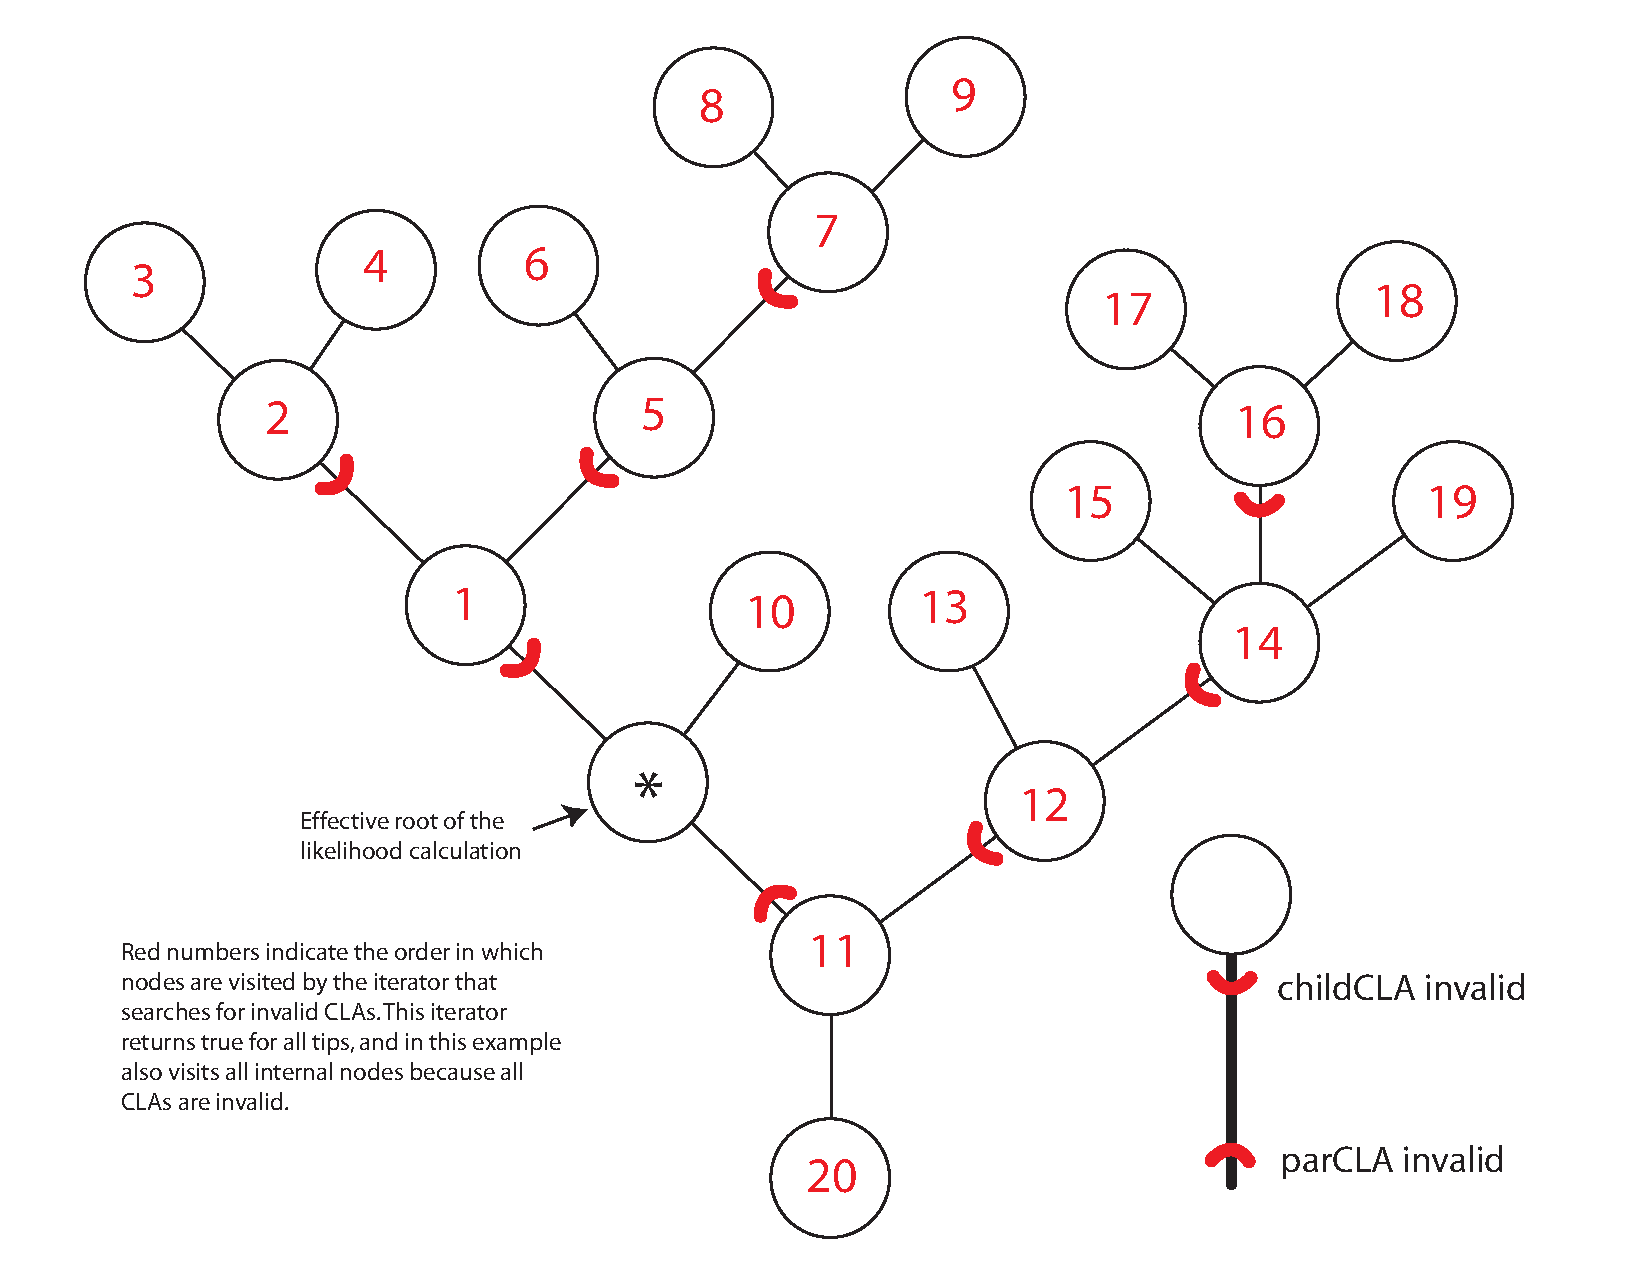
\includegraphics[scale=0.6]{ConditionalLikelihoodArrays/EffectiveRoot.pdf}\hfil
\caption{Order in which nodes are visited by the effective\_postorder\_edge\_iterator in the process of building a stack of nodes for which the TreeLikelihood::refreshCLA function is called.}
\label{edgeiterator}
\end{center}
\end{figure}

\subsection{TreeLikelihood::calcLnLFromNode}
If {\tt no\_data} is true, returns 0.0; otherwise, calls refreshCLA to update the CLAs that are invalid and then returns the value returned by the harvestLnL function. The effective\_postorder\_edge\_iterator is used to iterate through nodes for which refreshCLA needs to be called. This iterator first visits nodes in a centrifugal fashion away from the focal node, building a stack of nodes that need to have their CLAs recalculated. See Figure~\ref{edgeiterator} for an illustration of this process showing the order in which nodes are visited by the iterator in this first sweep to build the stack. Then, it pops nodes off this stack and hands them to the refreshCLA function. So CLAs are recalculated in a centripetal order (this would be equivalent to a postorder traversal if the likelihood root were equal to the actual root of the tree).

\subsection{TreeLikelihood::refreshCLA}
This function takes a reference to a focal node and a pointer to a node to avoid. It recalculates the CLA for the focal node in a direction away from the avoid node. The CLA is computed based on two nodes adjacent to the focal node, called firstNeighbor and secondNeighbor. If the path from the focal node to the likelihood root would go through the focal node's parent, then firstNeighbor is the leftmost child of the focal node and secondNeighbor is its right sibling, otherwise firstNeighbor is the parent of the focal node and secondNeighbor is the leftmost child that is not the avoid node. The necessary transition probability matrices are computed using one of two functions: calcPMat is used for internal nodes and calcPMatTranspose is used for tips. One of three functions (calcCLANoTips, calcCLAOneTip, calcCLATwoTips) is then called depending on the status of firstNeighbor and secondNeighbor. If secondNeighbor has siblings that are not equal to the avoided node, then the focal node represents a polytomy and either conditionOnAdditionalTip or conditionOnAdditionalInternal must be called for each extra sibling. Figure~\ref{edgeiterator} illustrates the CLAs that would be recomputed by this function in an example tree where the likelihood root is not equal to the actual root and no CLAs are currently valid.

\subsection{TreeLikelihood::calcPMat}

This function defers everything to calcPMatCommon.
\partition{First argument is now the subset index.}

\subsection{TreeLikelihood::calcPMatCommon}

Creates a vector of scaled edge lengths, each element of which is the edge length multiplied by a relative rate mean. It then passes a pointer to the beginning of this vector to the model's calcPMatrices function to do the work.
\partition{First argument is now the subset index.}

\subsection{TreeLikelihood::calcPMatTranspose}
\partition{First argument is now the subset index.}

\subsection{TreeLikelihood::calcCLAOneTip}

\subsection{TreeLikelihood::calcCLATwoTips}

\subsection{TreeLikelihood::conditionOnAdditionalTip}

\subsection{TreeLikelihood::conditionOnAdditionalInternal}

\subsection{TreeLikelihood::harvestLnL}

By the time harvestLnL is called, all CLAs are up-to-date. Normally, the sole argument is an EdgeEndpoints object in which the focal node is specified to be the likelihood root and the focal neighbor is NULL. In this case, the focal neighbor is set to be the parent of the focal node. The refreshCLA function is then called to refresh the childCLA of the focal node (i.e. its parent is specified as the avoid node). A new ConstEdgeEndpoints object is created and passed to harvestLnLFromValidEdge for processing.

\subsection{TreeLikelihood::harvestLnLFromValidEdge}

This function computes the log-likelihood (and site likelihoods if {\tt store\_site\_likes} is true) over all patterns. It is assumed that the focal node is an internal node. If the focal neighbor is a tip node, then the overall likelihood for pattern $k$ is
\begin{eqnarray*}
L_k & = & \sum_r \sum_{s_f} \pi_{s_f} P(s_f|s_n,r) L(f|s_f,r),
\end{eqnarray*}
where $L(f|s_f,r)$ is the likelihood conditional on state $s_f$ at the focal node for rate $r$, $\pi_{s_f}$ is the relative frequency of state $s_f$, and $P_{s_n|s_f,r}$ is the transition probability of ending in state $s_n$ given starting state $s_f$ for rate $r$. Note that Phycas uses the transition matrix backwards here ($P_{s_f|s_n,r}$ instead of $P_{s_n|s_f,r}$), which is ok as long as the model is time-reversible (and it must be time-reversible if the focal neighbor is a tip).

If the focal neighbor is an internal node, then the overall likelihood for pattern $k$ is instead
\begin{eqnarray*}
L_k & = & \sum_r \sum_{s_f} L(f|s_f,r) \left\{ \sum_{s_n} \pi_{s_f} P(s_n|s_f,r) L(n|s_n,r) \right\},
\end{eqnarray*}
where $L(f|s_f,r)$ is the likelihood conditional on state $s_f$ at the focal node for rate $r$, $L(n|s_n,r)$ is the likelihood conditional on state $s_n$ at the focal {\em neighbor} node for rate $r$, $\pi_{s_f}$ is the relative frequency of state $s_f$, and $P_{s_n|s_f,r}$ is the transition probability of ending in state $s_n$ given starting state $s_f$ for rate $r$. The quantity $\pi_{s_f} P(s_n|s_f,r)$ is precalculated and stored in {\tt piP[r][s\_f][s\_n]}, where {\tt piP} is a 3-dimensional temporary matrix. This is done to avoid recalculating the product of state frequency and transition probability for each pattern. This also explains why the $\pi_{s_f}$ is inside the $s_n$ loop.

For pinvar models, there is additional code to compute the likelihood of a pattern given that it is invariable. This work is only done if the pattern is potentially constant. There is also code for computing the correction for underflow. Finally, to obtain the site log-likelihood, the log-likelihood for each pattern is multiplied by the count for that pattern.



\chapter{Parameters and moves} 

A \term{move} in \phycas\ involves a Metropolis-Hastings update mechanism, whereas a \term{parameter} uses slice sampling.

%%%%%%%%%%%%%%%%%%%%%%%%%%%%%%%%%%%%%%%%%%%%%%%%%%%%%%%%%%%%%%
%%%%%%%%%%%%%%%%%%%%%%%%%%%%%%%%%%%%%%%%%%%%%%%%%%%%%%%%%%%%%%
\section{Adding a new move}
%%%%%%%%%%%%%%%%%%%%%%%%%%%%%%%%%%%%%%%%%%%%%%%%%%%%%%%%%%%%%%
%%%%%%%%%%%%%%%%%%%%%%%%%%%%%%%%%%%%%%%%%%%%%%%%%%%%%%%%%%%%%%

\begin{enumerate}
\item Create header (*.hpp) and source code (*.cpp) files for your move. The easiest way to do this is to copy the files for an existing move. Here is the basic boilerplate code for the header file:
\begin{verbatim}
#if ! defined(MY_NEW_MOVE_HPP)
#define MY_NEW_MOVE_HPP

#include <boost/weak_ptr.hpp>		// for boost::weak_ptr
#include "phycas/src/mcmc_updater.hpp"	// for base class MCMCUpdater

class MCMCChainManager;
typedef boost::weak_ptr<MCMCChainManager>  ChainManagerWkPtr;

namespace phycas
{

/*----------------------------------------
|   Description of what MyNewMove does.
*/
class MyNewMove : public MCMCUpdater
    {
    public:
                MyNewMove();
        virtual ~MyNewMove();
        bool    update();
    };
}  // namespace phycas
\end{verbatim}
And here is the corresponding minimal boilerplate for the source code file:
\begin{verbatim}
namespace phycas
{
/*----------------------------------------
|   MyNewMove constructor.
*/
MyNewMove::MyNewMove()
  {
  }

/*----------------------------------------
|   MyNewMove destructor.
*/
MyNewMove::~MyNewMove()
  {
  }

/*----------------------------------------
|   Description of update method.
*/
bool NielsenMappingMove::update()
    {
    // code for performing the update goes here
    return true;
    }
} // namespace phycas

\end{verbatim}
\item Write the constructor, destructor, and \method{update} member function, creating helper methods as necessary. The \method{update} method should return true if it changes the model, false if it leaves everything untouched (e.g. a Metropolis-Hastings proposal that is rejected). Note that because \class{MyNewMove} is derived from \class{MCMCUpdater}, it has access to the following shared pointers (as well as the other public and protected data members of the \class{MCMCUpdater} class):
\begin{itemize}
\item \shptr{tree} points to the \class{Tree} object
\item \shptr{tree\_manipulator} points to the \class{TreeManip} object
\item \shptr{model} points to the \class{Model} object
\item \shptr{likelihood} points to the \class{TreeLikelihood} object
\item \shptr{rng} points to the \class{Lot} (pseudorandom number generator) object
\end{itemize}
\item In \pathname{updater\_pymod.cpp}, add a Boost Python entry so that your new move can be called from Python code:
\begin{verbatim}
#include "phycas/src/my_new_move.hpp"
...
class_<phycas::MyNewMove, bases<phycas::MCMCUpdater>, 
  boost::noncopyable, boost::shared_ptr<phycas::MyNewMove> >("MyNewMove") 
  .def("update", &phycas::MyNewMove::update)
  ;
\end{verbatim}
\item Add the new move to the \method{setupChain} function of \class{MCMCManager}
\end{enumerate}

%%%%%%%%%%%%%%%%%%%%%%%%%%%%%%%%%%%%%%%%%%%%%%%%%%%%%%%%%%%%%%
%%%%%%%%%%%%%%%%%%%%%%%%%%%%%%%%%%%%%%%%%%%%%%%%%%%%%%%%%%%%%%
\section{Larget-Simon LOCAL move}
%%%%%%%%%%%%%%%%%%%%%%%%%%%%%%%%%%%%%%%%%%%%%%%%%%%%%%%%%%%%%%
%%%%%%%%%%%%%%%%%%%%%%%%%%%%%%%%%%%%%%%%%%%%%%%%%%%%%%%%%%%%%%

%
% Figure "MBTA"
%
%\clearpage
%\begin{figure}
%\centering
%\includegraphics[scale=0.5]{Figures/MBTA.eps}
%\label{MBTA}
%\caption{\small Map of the Massachusetts Bay Transit Authority subway system is a good example of a model. Is is an abstraction of reality that is nevertheless much more useful (for the purpose of using the subway system) than a very realistic map of the region.}
%\end{figure}


\chapter{Distribution checklist} 

\section{Building Phycas on Ubuntu 10.04}

\begin{enumerate}
\item Prepare operating system for building phycas
\begin{verbatim}
sudo apt-get install g++
sudo apt-get install python-dev
sudo apt-get install autoconf
sudo apt-get install subversion
sudo apt-get install curl
sudo apt-get install git-core
sudo apt-get install xsel
\end{verbatim}
%
\item Download \pathname{ncl-2.1.13.tar.gz} from \url{http://sourceforge.net/projects/ncl/}
\begin{verbatim}
cd $HOME
tar zxvf ncl-2.1.13.tar.gz
cd ncl-2.1.13
./configure
make
sudo make install
\end{verbatim}
Alternatively, download and build NCL from SourceForge Subversion checkout
\begin{verbatim}
cd $HOME
mkdir ndev
cd ndev
mkdir v2.1
svn co https://ncl.svn.sourceforge.net/svnroot/ncl/branches/v2.1 v2.1
cd v2.1
sh ./bootstrap.sh
./configure
make
sudo make install
\end{verbatim}
%
\item Download \pathname{boost\_1\_42\_0.tar.gz} from \url{http://www.boost.org/}
\begin{verbatim}
cd $HOME
tar zxvf boost_1_42_0.tar.gz
\end{verbatim}
%
\item Build bjam executable.
The following should create a new directory 
containing the bjam executable. 
The name of the directory will depend on whether your version of g++ is configured
to build for 32 or 64 bits. 
The directory created should be:\\
\pathname{\$HOME/boost\_1\_42\_0/tools/jam/src/bin.linuxx86}\\
or \\
\pathname{\$HOME/boost\_1\_42\_0/tools/jam/src/bin.linuxx86\_64} \\
con):
\begin{verbatim}
cd $HOME/boost_1_42_0/tools/jam/src
./build.sh
\end{verbatim}
%
\item Download and build phycas
\begin{verbatim}
cd $HOME
mkdir pdev
cd pdev
git clone git@github.com:mtholder/Phycas.git
cd Phycas
\end{verbatim}
%
\item Create file \pathname{\$HOME/pdev/Phycas/go.sh} to contain the following text:
\begin{verbatim}
#!/bin/bash

export OSTYPE="linux"
export BOOST_ROOT="$HOME/boost_1_42_0"
export PATH="${PATH}:$BOOST_ROOT/tools/jam/src/bin.linuxx86"
export BOOST_BUILD_PATH="${BOOST_ROOT}/tools/build/v2"
export PHYCAS_ROOT="$HOME/pdev/trunk"
export NCL_INSTALL_DIR="/usr/local"
export NCL_ALREADY_INSTALLED=1
bjam release
\end{verbatim}

Note that if building bjam created a 64 bit version then you will have to use
\begin{verbatim}
export PATH="${PATH}:$BOOST_ROOT/tools/jam/src/bin.linuxx86_64"
\end{verbatim}
to setup the correct path

%
\item Make \pathname{\$HOME/pdev/Phycas/go.sh} executable and build phycas
\begin{verbatim}
cd $HOME/pdev/trunk
chmod +x go.sh
./go.sh
\end{verbatim}
%
\item Prepare libraries for dynamic loading
\begin{verbatim}
/sbin/ldconfig $HOME/pdev/Phycas/phycas/Conversions /usr/local/lib/ncl
\end{verbatim}
(you may have to run this via sudo).
%
\item Create tar file of phycas distribution:
\begin{verbatim}
cd $HOME/pdev/trunk
python build_phycas_tarball.py
\end{verbatim}
%
\item Locate the python dist-packages directory:
\begin{verbatim}
python -c "from distutils.sysconfig import get_python_lib; print get_python_lib()"
\end{verbatim}
%
\item Assuming previous step revealed that the python dist-packages directory is \pathname{/usr/lib/python2.6/dist-packages}, move the tar file there and unpack:
\begin{verbatim}
cd /usr/lib/python2.6/dist-packages
sudo tar xvf "$HOME/pdev/trunk/phycas_distr.tar"
\end{verbatim}
%
\item See if phycas can be loaded into python:
\begin{verbatim}
python
>>> from phycas import *
\end{verbatim}

\subsection*{Preparing source distribution for the \url{phycas.org} web site}
The following command will create a \pathname{dist} directory inside of which is a \pathname{Phycas-1.2.0.tar.gz} file. The ``1.2.0'' part is obtained from \pathname{phycasver.txt}, so make sure that is correct first. The shell script first creates MANIFEST.in by concatenating MANIFEST.common and MANIFEST.linux. Subsequently, the distutils sdist command is used to create the distribution including all files listed in MANIFEST.in.
\begin{verbatim}
cd $HOME/pdev/Phycas
./build_linux_source_distr.sh
\end{verbatim}

\subsection*{Making python less painful}
bpython and ipython allow for tab completion and other have other helpful features that make phycas less painful to work with.

\subsubsection*{setuptools}
To install them, start by installing setuptools.  See \url{http://pypi.python.org/pypi/setuptools#cygwin-mac-os-x-linux-other}
This installation  will entail  grabbing the egg from \url{http://pypi.python.org/packages/2.6/s/setuptools/setuptools-0.6c11-py2.6.egg#md5=bfa92100bd772d5a213eedd356d64086}
and then installing it 
\begin{verbatim}
sh setuptools-0.6c11-py2.6.egg
\end{verbatim}
That may require sudo.

Setuptools should give you ``easy\_install'' on your path.
After that you should be able to run
\begin{verbatim}
easy_install bpython
easy_install ipython
\end{verbatim}
to install bpython and iPython.

\section{Building Phycas on Windows 7}

\subsection*{Preparing binary distribution for the \url{phycas.org} web site}
The following command will create a \pathname{dist} directory inside of which is a \pathname{Phycas-1.2.0.zip} file. The ``1.2.0'' part is obtained from \pathname{phycasver.txt}, so make sure that is correct first. The shell script first creates MANIFEST.in by concatenating MANIFEST.common and MANIFEST.windows. Subsequently, the distutils sdist command is used to create the distribution including all files listed in MANIFEST.in.
\begin{verbatim}
cd $HOME/pdev/Phycas
./build_windows_source_distr.sh
\end{verbatim}

\section{Building Phycas on Mac OS 10.6.4 (Snow Leopard)}

\end{enumerate}


\bibliography{developerguide}

%\appendix

%\include{Appendix1} 
%\include{Appendix2} 

%\include{index}
\end{document}

